\documentclass[fleqn]{jbook}
\usepackage{physpub}

\begin{document}
\begin{question}{専攻 問題3}{}

Maxwellは、いくつかの実験事実から4つの方程式(Maxwell方程式)

\begin{eqnarray}
  \nabla \cdot \vec{E} = \frac {\rho}{\varepsilon_{0}} 
  \ilabel{Q01}
\end{eqnarray} 
\begin{eqnarray}
  \nabla \cdot \vec{B} = 0
  \ilabel{Q02}
\end{eqnarray} 
\begin{eqnarray}
  \nabla \times \vec{E} = - \frac{\partial \vec{B}}{\partial t}
  \ilabel{Q03}
\end{eqnarray} 
\begin{eqnarray}
  \frac{1}{\varepsilon_{0} \mu_{0}}\nabla \times \vec{B} = %
  \frac{\vec{j}}{\varepsilon_{0}} + \frac{\partial \vec{E}}{\partial t}      
  \ilabel{Q04}
\end{eqnarray} 

を与え、電磁気学を完成させた。ただし$\vec{E}$は電場、$\vec{B}$は磁束密
度、$\rho$は電荷密度、$\vec{j}$は電流密度、$\varepsilon_{0}$は真空の誘電率、
$\mu_{0}$は真空の透磁率で、以下では真空中の電磁場のみを考える。

\begin{subquestions}
\SubQuestion
  式\iref{Q01}はGaussの法則を表す。
  \begin{subsubquestions}
  \SubSubQuestion
  閉じた中空の導体があると、導体の外部にある電荷が作る電場は、導体に囲
  まれた中空の導体には侵入できない。このことを、式\iref{Q01}を用いて証明せよ。
  ただし、中空の空間には、もともと電荷は存在しなかったものとする。

  \SubSubQuestion
  $R_{1}$および$R_{2}$($R_{1}>R_{2}$)の半径をもつ2個の同心の中空導体球
  を用いて、Gaussの法則を実験的に検証したい。原理的にどのような手順で何
  を測定すれば良いか、答えよ。
  \end{subsubquestions}

\SubQuestion
  Maxwell方程式から電磁波の存在が予言される。
  \begin{subsubquestions}
  \SubSubQuestion
  電荷の保存則を用いて、Amp\`{e}reの法則、すなわち、「ある閉曲線が囲む
  定常電流$I$によって生じる磁場$\vec{B}/\mu_{0}$をその閉曲線に沿って線
  積分すると、$I$に等しい」を非定常電流の場合に一般化し、式\iref{Q04}を導け。

  \SubSubQuestion
  ある瞬間に電流密度$\vec{j}$が局所的に発生し、短時間で消滅したとする。
  その後の$\vec{B}$と$\vec{E}$はどのように変動するか。
  式\iref{Q03}と\iref{Q04}を用い
  て、直観的に説明せよ。

  \SubSubQuestion
  電荷や電流の分布が無い場合、真空中を伝播する電磁波が存在することを導
  け。またその速度を、設問に与えられた量を用いて示せ。
  \end{subsubquestions}

\SubQuestion
  適当なスカラー場(スカラーポテンシャル)$\phi$とベクトル場(ベクトル
  ポテンシャル)$\vec{A}$を導入することにより、
  \[
    \vec{B} = \nabla \times \vec{A} , \hspace{10mm}
    \vec{E} = - \nabla \phi - \frac { \partial \vec{A} } { \partial t }
  \]
  と表せることを示せ。

\end{subquestions}

\end{question}
\begin{answer}{専攻 問題3}{}

\begin{subanswers}
\SubAnswer
  \begin{subsubanswers}
  \SubSubAnswer
    \parbox[t]{100mm}{
   中空の空間には電荷が存在しない($\rho=0$)ので、\iref{Q01}より$\Div \vec{E}=0
   $。\\
   従って、中空の空間には電場の湧き出しやすいこみがなく、中空の空間に
   電場が侵入するとすれば、電気力線は右図のように導体内側表面の2点A、
   Bを結ぶことになる。\\
   すると、2点A、Bの間に電位差が生じることになるが、これは導体の各部
   分の電位が等しいことに反する。\\
   よって、中空の空間には電場は侵入できない。\\
   (ちなみに、導体の各部分の電位が等しいことは、電荷の移動が終了した
   状態では導体内部に電場が存在しないということから結論される)
   
    
    
  \SubSubAnswer
   
   (i)より、導体球1の中空の空間には電場が侵入できないので、導体球1と
   導体球2の電位は等しいはずである。よって、導体球の外に置いた電荷の
   位置や量を変えても、導体球1と2の間の電位差が常に0であることを確
   かめればよい。}
   \parbox[t]{50mm}{
   
   \begin{center}
    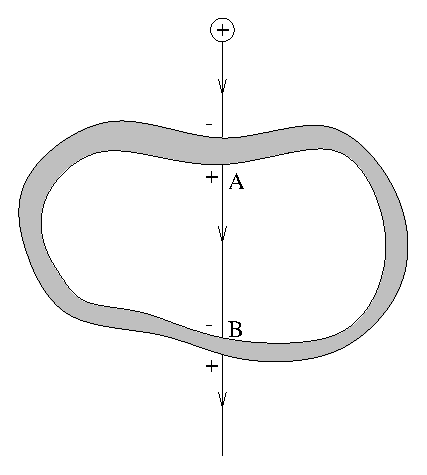
\includegraphics[clip,height=36mm,width=45mm]{1998phy3-1.eps}
   \end{center}
%   \vspace{1mm}
   \begin{center}
     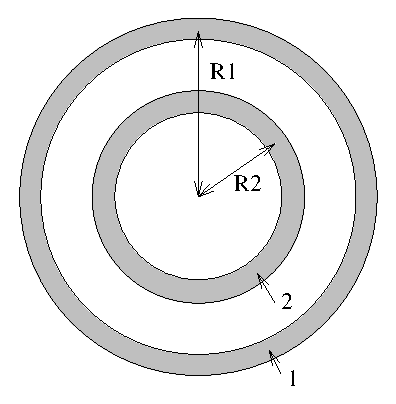
\includegraphics[clip,height=30mm]{1998phy3-2.eps}
   \end{center}
   }
  \end{subsubanswers}
 
 \SubAnswer
  \begin{subsubanswers}
  \SubSubAnswer
    $S$を任意の閉曲面、$V$を$S$の内部の領域として、電荷保存則は
    \begin{eqnarray}
      \int_{S} \vec{j} \cdot \vec{n} {\d{S}} = -\frac{d}{dt}
      \int_{V} \rho {\d{V}}
      \ilabel{Q1}
    \end{eqnarray}
    定常電流の時は
    \[
      \int_{S} \vec{j} \cdot \vec{n} {\d{S}} = 0
    \]
    が成立するが、非定常電流の時は
    \begin{eqnarray}
    \ilabel{Q3}
      \frac{d}{dt} \int_{V} \rho {\d{V}} = 
      \frac{d}{dt} \int_{V} \varepsilon_0 \nabla \cdot \vec{E} {\d{V}} = 
      \frac{d}{dt} \int_{S} \varepsilon_0 \vec{E} \cdot \vec{n} {\d{S}} = 
      \int_{S} \varepsilon_0 \frac{\partial \vec{E}}{\partial t} \cdot %
      \vec{n} {\d{S}}
    \end{eqnarray}
    \iref{Q3}を\iref{Q1}に代入して
    \[
      \int_{S} \left( \vec{j} + \varepsilon_0 \frac{\partial \vec{E}} %
      {\partial t} \right) \cdot \vec{n} {\d{S}} = 0
    \]
    が成立する。\\
    従って、定常電流のときのAmp\`{e}reの法則
    \begin{eqnarray}
      \oint_{C} \vec{B} \cdot \vec{r} = %
      \mu_{0} \int_{S'} \vec{j} \cdot \vec{n} {\d{S}}
      \ilabel{Q4}
    \end{eqnarray}
    を非定常電流の場合に一般化するには、
    \[
      \vec{j} \rightarrow %
      \vec{j} + \varepsilon_0 \frac{\partial \vec{E}}{\partial t}
    \]
    と置き換えて、
    \begin{eqnarray}
      \oint_{C} \vec{B} \cdot {\d{\vec{r}}} = %
      \mu_{0} \int_{S'} \left( \vec{j} + \varepsilon_0 \frac %
      {\partial \vec{E}}{\partial t} \right) \cdot \vec{n} {\d{S}}
      \ilabel{Q5}
    \end{eqnarray}
    とすればよい。
    Stokesの定理より
    \[
      \oint_{C} \vec{B} \cdot {\d{\vec{r}}} = %
      \int_{S'} \nabla \times \vec{B} \cdot \vec{n} {\d{S}}
    \]
    であるから、\iref{Q5}は
    \[
      \int_{S'} \nabla \times \vec{B} \cdot \vec{n} {\d{S}} = %
      \int_{S'} \mu_{0} \left( \vec{j} + \varepsilon_0 \frac %
      {\partial \vec{E}}{\partial t} \right) \cdot \vec{n} {\d{S}}
    \]
    となる。$S'$は任意なので
    \[
      \nabla \times \vec{B} = \mu_{0} \left( \vec{j} + %
      \varepsilon_0 \frac {\partial \vec{E}}{\partial t} \right)
    \]
    これで、\iref{Q04}が導かれた
  \SubSubAnswer
    局所的な$\vec{j}$が一瞬生じると、\iref{Q04}によって近傍に$\vec{B}$
    が生じ、$\vec{B}$の変化があるので\iref{Q03}によって近傍に$\vec{E}$が生じ、
    $\vec{E}$の変化があるので、再び\iref{Q04}によって近傍に$\vec{B}$が生じる\\
    $\vec{j}$が消滅した後\iref{Q02}も、引き続き\iref{Q03},\iref{Q04}
    によって$\vec{E}$,$\vec{B}$の
    変化がそれぞれ近傍に$\vec{E}$、$\vec{B}$を生むので、電磁波のパルスが
    空間を伝わっていく。

  \SubSubAnswer
    $\rho=0,\ \vec{j}=0$のとき、Maxwell方程式は
    \begin{eqnarray}
      \Div \vec{E} = 0
      \ilabel{c1}
    \end{eqnarray}
    \begin{eqnarray}
      \Div \vec{B} = 0
      \ilabel{c2}
    \end{eqnarray}
    \begin{eqnarray}
      \Rot \vec{E} = - \frac { \partial \vec{B} } { \partial t}
      \ilabel{c3}
    \end{eqnarray}
    \begin{eqnarray}
      \Rot \vec{B} = \varepsilon_{0}\mu_{0}\frac{\partial \vec{E}}{\partial t}
      \ilabel{c4}
    \end{eqnarray}
    となる。
    \iref{c3}のrotをとると
    \[
      \nabla \times \nabla \times \vec{E} =
      \nabla \left( \nabla \cdot \vec{E} \right) - \nabla^{2} \vec{E} 
    \]
    を使って
    \[
      \Grad \Div \vec{E} - \nabla^{2} \vec{E} =
      - \frac{\partial}{\partial t}\left( \Rot \vec{B} \right) 
    \]
    これに\iref{c1},\iref{c4}を代入すると
    \begin{eqnarray}
      \nabla^{2} \vec{E} = %
      \varepsilon_{0}\mu_{0}\frac{\partial^{2} \vec{E}}{\partial t^{2}}
      \ilabel{c5}
    \end{eqnarray}
    が得られる。同様に\iref{c4}のrotをとれば
    \begin{eqnarray}
      \nabla^{2} \vec{B} = %
      \varepsilon_{0}\mu_{0}\frac{\partial^{2} \vec{B}}{\partial t^{2}}
      \ilabel{c6}
    \end{eqnarray}
    が得られる。\\
    \iref{c5},\iref{c6}は波動方程式であるから、電磁場の存在が示された。
    位相速度は
    \[
      c = \frac{1}{\sqrt{\varepsilon_{0} \mu_{0}}}
    \]
    である。

  \SubSubAnswer
    $\Div \Grad=0$であるから、\iref{Q02}より
    \begin{eqnarray}
      \vec{B}=\Rot \vec{A}
      \ilabel{31}
    \end{eqnarray}
    なるベクトル場$\vec{A}$が存在することが分かる。\\
    \iref{31}を\iref{Q03}に代入すると

    \[
      \Rot \vec{E}= -\Rot \frac{\partial \vec{A}}{\partial t}
    \]

    \[
      \Rot \left( \vec{E} + \frac{\partial \vec{A}}{\partial t} \right) = 0 
    \]
    ところが$\Rot \Grad=0$であるから
    \[
     \vec{E} + \frac{\partial \vec{A}}{\partial t} = - \Grad \phi
    \]
    なるスカラー場$\phi$が存在することが分かる。
  \end{subsubanswers}
\end{subanswers}
\end{answer}


\end{document}
